\section{Metodologia}\label{sec:metodologia}

Esta seção apresenta a instanciação do método utilizada nos experimentos. Conforme discutido na Seção \ref{sec:kernel_pipeline}, as escolhas descritas a seguir (modelo, amostra, fontes, \textit{kernels} e transformações) não fazem parte do método e foram realizadas para demonstrar o seu funcionamento. Qualquer pipeline núcleo-transformação produz uma matriz semidefinida positiva e, consequentemente, uma pseudométrica, mas nada na forma do método garante que a geometria resultante diga algo sobre o modelo que a originou. A pergunta que orienta esta seção é, portanto: ``a geometria induzida reflete o comportamento do modelo?''.

Validar a geometria não significa mostrar que o espaço separa classes, visto que um espaço construído sobre as ativações de uma rede treinada separa classes quase por construção. A afirmação testada é que as distâncias do espaço preveem o que o modelo faz, isto é, qual classe ele decide, em quais amostras ele erra e quais categorias ele confunde. Por esse motivo, sempre que possível, a referência é algo que o próprio modelo produziu (a predição, o erro e a confusão), e não o rótulo do conjunto de dados. Além disso, as leituras são repetidas sobre doze conjuntos de dados, várias sementes e três arquiteturas, cada afirmação é reportada como a fração das execuções em que ela se sustenta e, onde o número de execuções permite, por teste pareado e intervalo de confiança (Subseção \ref{subsec:estatistica}), e toda leitura é acompanhada de uma referência de nulidade, ou piso (Subseção \ref{subsec:pisos}).

\subsection{Perguntas que orientam os experimentos}\label{subsec:perguntas}

A pergunta central se desdobra em nove perguntas, que determinam os experimentos e a ordem em que os resultados são apresentados na Seção \ref{sec:resultados}. Cada uma é respondida contra uma referência externa à geometria, visto que uma pergunta cuja resposta dependa apenas da própria geometria não pode ser respondida pelo método que a produziu.

\begin{enumerate}
    \item[\textbf{P1.}] \textit{A geometria reflete o comportamento do modelo?} As distâncias preveem qual classe o modelo decide, em quais amostras ele erra e quais classes ele confunde? A referência é o comportamento do próprio modelo, e o piso é a mesma construção sobre o modelo não treinado.

    \item[\textbf{P2.}] \textit{A composição acrescenta algo às fontes isoladas?} Se a matriz de Gram conjunta não superar a melhor fonte isolada, o produto de Hadamard seria apenas uma forma mais custosa de ler essa fonte. A comparação inclui, além das fontes isoladas, a composição aditiva com as mesmas fontes e a mesma normalização, pois só assim se testa se a forma \emph{multiplicativa} é o que acrescenta informação (Subseção \ref{subsec:experimentos}, terceira família).

    \item[\textbf{P3.}] \textit{O método se distingue de uma simples CKA?} A matriz de Gram do método é centrada e normalizada, o mesmo tipo de objeto sobre o qual a CKA opera. A pergunta não é respondida pelo valor do alinhamento, e sim pelo conteúdo: a parte da Gram que a CKA não enxerga carrega informação sobre o comportamento do modelo?

    \item[\textbf{P4.}] \textit{A energia espectral descreve como o modelo representa cada amostra?} O subespaço retido $V_r$ contém as direções que separam as decisões do modelo, e a energia que escapa dele, medida por $\widehat{E}_{\mathrm{ratio}}$, sinaliza as amostras em que o modelo erra?

    \item[\textbf{P5.}] \textit{Que informação espacial sobre as representações do modelo oferecem o campo de energia e os conjuntos de nível?} A pergunta tem três partes, reportadas separadamente: se a energia se concentra sobre o objeto (verificado pela máscara de segmentação), como a ordenação espacial se relaciona à evidência da decisão (verificado por deleção) e se os conjuntos de nível reúnem as regiões que o modelo representa de forma semelhante.

    \item[\textbf{P6.}] \textit{Por que esta amostra foi classificada de forma diferente daquela?} Essa é a forma local e contrastiva do método. A amostra comparada é um contrafactual da amostra explicada, no sentido da Seção \ref{sec:referencial}, e a resposta é um ranking de atributos ou de regiões. A validação é feita por intervenção sobre a entrada: levar os primeiros atributos do ranking ao valor do contrafactual deve mudar a decisão do modelo.

    \item[\textbf{P7.}] \textit{As leituras dependem do modelo?} As fontes da Subseção \ref{subsec:fontes} não fazem referência à convolução, e o mesmo código é aplicado a um perceptron multicamadas, a uma rede convolucional e a um transformador. Na sua forma mais forte, a pergunta é se o método é de fato modelo-agnóstico, e ela é respondida aplicando-o a uma árvore de decisão.

    \item[\textbf{P8.}] \textit{Em que profundidade a decisão se forma?} As leituras por bloco produzem uma datação da decisão, que é comparada a uma datação independente, obtida por intervenção $do(\cdot)$ sobre os estados internos.

    \item[\textbf{P9.}] \textit{As distâncias refletem uma organização semântica que o modelo nunca viu?} As perguntas anteriores comparam a geometria ao comportamento do próprio modelo. Esta compara-a a uma referência semântica externa a ele: a hierarquia de classes da base (a espécie de cada raça no Oxford-IIIT Pet e a superclasse de cada classe no CIFAR-100), que não entra no treinamento. Como um modelo que confunde classes semanticamente próximas já carrega parte da hierarquia no seu comportamento, a leitura é comparada também à hierarquia contida na confusão do próprio modelo.
\end{enumerate}

P1 é a pergunta da qual as demais dependem: se a geometria não refletir o comportamento do modelo, as demais leituras descreveriam um espaço sem relação com ele. As perguntas P1 a P4 e P9 tomam cada amostra como um objeto, P5 aplica-se apenas às imagens, P6 e P8 são respondidas com intervenções, sobre a entrada e sobre os estados internos, e P7 repete as leituras sobre outros modelos.

\subsection{Bases de dados}\label{subsec:dados}

O primeiro conjunto de bases reúne dez bases tabulares do OpenML \citep{Vanschoren2014}, descritas na Tabela \ref{tab:bases}, sete das quais integram o OpenML-CC18 \citep{Bischl2021}. Os critérios de seleção foram fixados antes das medições: todas são multiclasse (de 3 a 26 classes), possuem ao menos duas mil amostras e não possuem classes com pouquíssimos exemplos. Os arquivos foram lidos das fontes originais que o OpenML publica (o repositório da UCI e, para a \texttt{dna}, a versão do StatLog), com os rótulos codificados na mesma ordem lexicográfica do OpenML. A única diferença de forma é a \texttt{satimage}, com 6\,435 amostras nos arquivos originais. A \texttt{covertype} é subamostrada de forma estratificada para 30\,000 amostras. Os atributos são padronizados pelas estatísticas do treino, e a partição é estratificada em 70\% para treino, 10\% para validação e 20\% para teste.

\begin{table}[pos=htbp]
\centering
\caption{Bases tabulares utilizadas, com o identificador no OpenML, o número de amostras (após a subamostragem, no caso da \texttt{covertype}), de atributos e de classes, e a referência de origem. A última coluna indica as bases que integram o OpenML-CC18 \citep{Bischl2021}.}
\label{tab:bases}
\footnotesize
\setlength{\tabcolsep}{4pt}
\begin{tabular}{l r r r r l c}
\hline
Base & OpenML & Amostras & Atributos & Classes & Origem & CC18 \\
\hline
\texttt{letter} & 6 & 20\,000 & 16 & 26 & \citet{FreySlate1991} & sim \\
\texttt{pendigits} & 32 & 10\,992 & 16 & 10 & \citet{UCIPendigits} & sim \\
\texttt{optdigits} & 28 & 5\,620 & 64 & 10 & \citet{AlpaydinKaynak1998} & sim \\
\texttt{satimage} & 182 & 6\,435 & 36 & 6 & \citet{UCISatimage} & sim \\
\texttt{segment} & 36 & 2\,310 & 19 & 7 & \citet{UCISegment} & não \\
\texttt{har} & 1478 & 10\,299 & 561 & 6 & \citet{Anguita2013} & sim \\
\texttt{mfeat-factors} & 12 & 2\,000 & 216 & 10 & \citet{vanBreukelen1998} & sim \\
\texttt{gas-drift} & 1476 & 13\,910 & 128 & 6 & \citet{Vergara2012} & não \\
\texttt{dna} & 40670 & 3\,186 & 180 & 3 & \citet{Michie1994} & sim \\
\texttt{covertype} & 1596 & 30\,000 & 54 & 7 & \citet{Blackard1999} & não \\
\hline
\end{tabular}
\end{table}

O segundo conjunto é o Oxford-IIIT Pet \citep{Parkhi2012}, com 7\,349 fotografias de 37 raças de gatos e cachorros, a partição oficial em 3\,680 imagens de \textit{trainval} e 3\,669 de teste e uma máscara de segmentação por imagem. As imagens são recortadas no centro em $128\times128$ píxeis, e a máscara recebe o mesmo recorte. A máscara nunca entra no treinamento nem na construção das matrizes de Gram: ela é a verdade externa contra a qual as leituras espaciais são verificadas. A base impõe um regime de dados escassos, com cerca de noventa imagens de treino por raça. A espécie de cada raça (12 de gatos e 25 de cachorros), que consta da lista oficial da base, é a referência semântica de P9.

O terceiro conjunto é o CIFAR-100 \citep{Krizhevsky2009}, com 60\,000 imagens de $32\times32$ píxeis em 100 classes e a partição oficial em 50\,000 de treino e 10\,000 de teste. A base é a mais utilizada na literatura de similaridade de representações \citep{Kornblith2019} e acrescenta ao Pet um regime oposto, com muitas classes e muitos exemplos por classe. As 100 classes são agrupadas oficialmente em 20 superclasses de cinco classes cada. O modelo é treinado apenas nas classes finas, e as superclasses servem somente como referência semântica de P9.

Todas as bases têm mais de duas classes, e isso é deliberado. Em uma tarefa binária, a margem contrastiva definida adiante se reduz à diferença entre dois logits, e trocar a predição inverte o sinal do gradiente em toda a rede, de modo que qualquer \textit{kernel} sensível a sinal separa as duas populações por construção. As matrizes de Gram por objeto são construídas sobre um subconjunto balanceado do teste, sorteado com semente fixa e sem aumento de dados, com $n \approx 500$ objetos nas bases tabulares e no Pet e $n = 1\,000$ (dez por classe) no CIFAR-100.

\subsection{Modelos e treinamento}\label{subsec:modelo}

São utilizadas três arquiteturas com a mesma estrutura de sondagem: sete estados, denotados por \texttt{stem} e \texttt{b1} a \texttt{b6}, em que o ponto de sondagem é sempre a saída do bloco. Nas bases tabulares, o modelo é um perceptron multicamadas residual com seis blocos de largura 256, da forma $h_{\ell} = \mathrm{ReLU}\bigl(\mathrm{BN}(W_2\,\mathrm{ReLU}(\mathrm{BN}(W_1 h_{\ell-1}))) + h_{\ell-1}\bigr)$, seguidos de uma cabeça linear. Nas imagens, o primeiro modelo é uma ResNet \citep{He2016} de três estágios, com dois blocos residuais cada e larguras de 64, 128 e 256 canais. O segundo é um transformador de visão com tokenizador convolucional \citep{Hassani2021}, em que o estado de cada bloco é mantido na forma espacial $(C, H, W)$ e as projeções do bloco são convoluções $1\times1$, idênticas a camadas lineares por \textit{token}. Assim, as mesmas fontes são extraídas das duas redes de imagem sem nenhuma alteração do código. No CIFAR-100 é utilizada a mesma ResNet, com passo 1 na convolução de entrada, de modo que os estados ficam em $32\times32$, $16\times16$ e $8\times8$ posições.

Todos os modelos são treinados do zero, com os hiperparâmetros da Tabela \ref{tab:hiperparametros}, com cinco sementes por base tabular e oito por arquitetura nas imagens. Essa escolha não é acessória: o piso das leituras de comportamento é o mesmo modelo com os pesos da inicialização, gravados antes da primeira época, e uma inicialização pré-treinada já carregaria geometria aprendida. Para modelos pré-treinados, o piso equivalente é a mesma rede com os pesos reinicializados, como nos testes de sanidade de mapas de saliência \citep{Adebayo2018}, de modo que a escolha de treinar do zero é uma conveniência do protocolo e não uma restrição do método. No Oxford-IIIT Pet, a ResNet atinge acurácia de teste de $0{,}670 \pm 0{,}010$ e o transformador, $0{,}438 \pm 0{,}011$. No CIFAR-100, a ResNet atinge $0{,}748 \pm 0{,}002$. A diferença é esperada para um transformador treinado do zero com poucos dados, e as comparações do método são sempre relativas ao piso do próprio modelo.

\begin{table}[pos=htbp]
\centering
\caption{Hiperparâmetros de treinamento. O aumento de dados é aplicado apenas ao conjunto de treino, e a amostra utilizada nas matrizes de Gram e em todas as leituras não é aumentada.}
\label{tab:hiperparametros}
\small
\setlength{\tabcolsep}{4pt}
\begin{tabular}{>{\raggedright\arraybackslash}p{0.19\linewidth} >{\raggedright\arraybackslash}p{0.36\linewidth} >{\raggedright\arraybackslash}p{0.36\linewidth}}
\hline
 & Bases tabulares (MLP residual) & Imagens (ResNet e transformador) \\
\hline
Otimizador & Adam & SGD com momento de Nesterov $0{,}9$ (ResNet) e AdamW (transformador) \\
Taxa de aprendizado & $10^{-3}$ & \textit{one-cycle}, máxima $0{,}05$ (ResNet) e $10^{-3}$ (transformador) \\
Decaimento de pesos & $10^{-4}$ & $5\times10^{-4}$ (ResNet) e $0{,}05$ (transformador) \\
Épocas & até 100, com parada antecipada (paciência 15) & 120 (Pet) e 60 (CIFAR-100) \\
Tamanho do lote & 256 & 64 \\
Função de perda & entropia cruzada, suavização $0{,}05$ & entropia cruzada, suavização $0{,}05$ (ResNet) e $0{,}1$ (transformador) \\
Aumento de dados & nenhum & espelhamento horizontal, recorte aleatório, variação de cor e apagamento aleatório \\
Mistura de amostras & nenhuma & \textit{mixup} ou \textit{cutmix} em metade dos lotes \\
Sementes & 0 a 4 & 0 a 7 \\
\hline
\end{tabular}
\end{table}

\subsection{As três fontes indexadas por objeto}\label{subsec:fontes}

Cada objeto $z_i$ é representado, no domínio produto da Definição \ref{def:tensor_sim}, por $d = 3$ fontes extraídas do mesmo bloco, que descrevem o estado do bloco, a sensibilidade da decisão a esse estado e os parâmetros que produzem esse estado.

A primeira fonte são as ativações ($A$), isto é, o estado de saída do bloco, reduzido por \textit{pooling} médio a uma grade comum de $4\times4$ posições e achatado como $A_i \in \mathbb{R}^{C \times P}$, com $P = 16$ nas imagens e $P = 1$ nos modelos tabulares.

A segunda fonte é o gradiente contrastivo ($\Omega$), a derivada, com respeito ao mesmo estado, da margem entre o logit de uma classe de referência e a média dos logits das demais,
\begin{equation}\label{eq:margem}
    m(z_i) = f_{c^\star}(z_i) - \frac{1}{Q-1}\sum_{c \neq c^\star} f_c(z_i),
\end{equation}
em que $Q$ é o número de classes.

Tomar $c^\star$ como a classe predita torna circulares as leituras referidas à predição, visto que o gradiente passa a carregar a própria predição. No perceptron, por exemplo, a classe predita explica 100\% da variação de $\Omega$ em \texttt{b6}. Por esse motivo, as leituras referidas ao comportamento utilizam um \textbf{alvo fixo}, isto é, a mesma classe de referência para todos os objetos. Representações sem geometria, como $\Omega$ no último bloco sob alvo fixo, são marcadas como indefinidas.

A terceira fonte são os parâmetros ativados ($W$), isto é, os filtros que o objeto de fato ativou. Sendo $W \in \mathbb{R}^{C \times C'}$ os pesos da camada de saída do bloco e $A_i[:,s]$ o vetor de ativações por canal na posição $s$,
\begin{equation}\label{eq:fonte_parametros}
    w_i[:,s] \;=\; W^\top A_i[:,s] \;\in\; \mathbb{R}^{C'},
    \qquad
    \langle w_i, w_j\rangle \;=\; \sum_{s=1}^{P} A_i[:,s]^\top (WW^\top)\, A_j[:,s] .
\end{equation}
Quando $P=1$ (modelos tabulares), a expressão se reduz a $A_i[:,1]^\top (WW^\top) A_j[:,1]$. Para $P>1$, a forma bilinear é aplicada posição a posição e somada. A matriz de Gram dos filtros é a mesma para todos os objetos e, portanto, não pode indexá-los. Na construção \eqref{eq:fonte_parametros}, ela reaparece como a forma bilinear da fonte, ponderada pela ativação de cada objeto.

\subsection{Construção das matrizes de Gram}\label{subsec:construcao}

Para cada bloco e cada fonte $l \in \{W, A, \Omega\}$, a matriz de Gram bruta é calculada com \textit{kernel} linear, recebe a transformação angular $T_a$ da Tabela \ref{tab:T_catalog} e é deslocada para o intervalo $[0,1]$. As três componentes são compostas pelo produto de Hadamard do Corolário \ref{cor:hadamard_form}, e o resultado é centrado e normalizado em traço:
\begin{equation}\label{eq:componente}
    \mathbf{G}_l \;=\; \frac{T_a(\widetilde{\mathbf{G}}_l) + \mathbf{J}}{2},
    \qquad
    \mathbf{G} \;=\; T_{\mathrm{tr}}\Bigl(T_c\bigl(\mathbf{G}_W \circ \mathbf{G}_A \circ
    \mathbf{G}_\Omega\bigr)\Bigr),
\end{equation}
em que $\mathbf{J} = \mathbf{1}\mathbf{1}^\top$. A partir de $\mathbf{G}$ é obtida a pseudodistância $d_{\mathbf{G}}^2(i,j) = G_{ii} + G_{jj} - 2G_{ij}$ da Equação \eqref{eq:gram_distance}. A Figura \ref{fig:gram_construcao} ilustra cada etapa.

Cada escolha responde a um problema concreto. O \textit{kernel} linear preserva a interação multiplicativa entre as fontes, enquanto, com \textit{kernels} gaussianos, o produto de Hadamard se reduz identicamente a uma soma das métricas das fontes. A normalização angular impede que a fonte de maior amplitude domine a composição: sem ela, a ordenação do produto concorda com a do gradiente entre $0{,}95$ e $1{,}00$. O deslocamento por $\mathbf{J}$, que é semidefinida positiva, evita que o produto de três cossenos em torno de zero torne a Gram conjunta numericamente diagonal, e o centramento remove a direção uniforme que esse deslocamento injeta no espectro. Pela Proposição \ref{prop:invariancia_distancias}, o centramento e a normalização em traço aplicados à Gram conjunta não alteram a ordem das distâncias. Eles afetam apenas as leituras espectrais. Já a normalização angular $T_a$ e o deslocamento por $\mathbf{J}$ são aplicados a cada fonte antes da composição e alteram a geometria. A sua contribuição é verificada por ablação (Subseção \ref{subsec:experimentos}, terceira família), e não assumida.

\begin{figure}[pos=htbp]
\centering
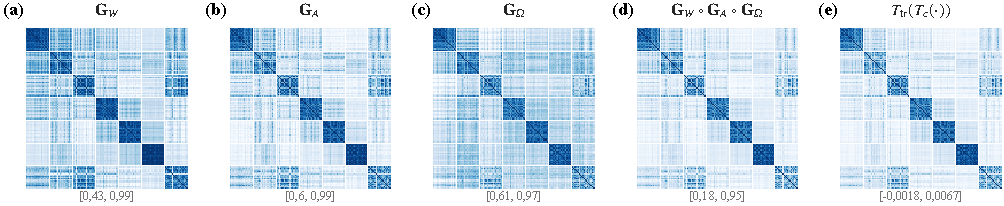
\includegraphics[width=\textwidth]{gram_construcao.pdf}
\caption{Construção da matriz de Gram, ilustrada sobre a base \texttt{segment} (sete classes, vinte amostras por classe), no bloco \texttt{b3} do perceptron multicamadas com alvo fixo. Da esquerda para a direita são apresentadas as matrizes de Gram componentes ($\mathbf{G}_W$, $\mathbf{G}_A$ e $\mathbf{G}_\Omega$), o produto de Hadamard que as compõe e a matriz de Gram após o centramento e a normalização em traço. Os objetos estão ordenados por classe, com as fronteiras entre as classes marcadas por linhas claras, e tons escuros indicam maior similaridade.}
\label{fig:gram_construcao}
\end{figure}

\subsection{Experimentos}\label{subsec:experimentos}

Os experimentos são divididos em cinco famílias, de acordo com a referência que cada uma utiliza, além da datação por intervenção.

A \textbf{primeira família} (P1 e P2) reúne as leituras da matriz de distância: a acurácia de $k$-vizinhos \textit{leave-one-out} contra a predição do modelo, a área sob a curva ROC da margem geométrica como preditora do acerto e a correlação de Spearman, no nível de classe, entre a proximidade geométrica dos pares de classes e a \textbf{confusão suave}, isto é, a probabilidade média que o modelo atribui à classe $b$ nas amostras da classe $a$, simetrizada e calculada sobre o teste inteiro. A \textbf{margem geométrica} de um objeto $i$ agrupa os objetos pela classe que o modelo \emph{prediz} e é
\begin{equation}\label{eq:margem_geometrica}
    \mu_i \;=\; \frac{\bar d_{i,\mathrm{viz}} - \bar d_{i,\hat y_i}}{\bar d_{i,\mathrm{viz}} + \bar d_{i,\hat y_i}},
\end{equation}
em que $\bar d_{i,c}$ é a distância média de $i$ aos objetos preditos na classe $c$, $\hat y_i$ é a predição de $i$ e $\bar d_{i,\mathrm{viz}}$ é a menor distância média às demais classes preditas. O rótulo verdadeiro entra apenas como a resposta a prever, isto é, o acerto, de modo que a margem é um sinal disponível em uso, sem acesso ao rótulo da amostra. Para saber o que a geometria acrescenta a sinais que não usam o método, a margem é comparada à probabilidade máxima do \textit{softmax} \citep{Hendrycks2017}, à margem entre os dois maiores \textit{logits}, ao \textit{trust score} \citep{Jiang2018} e à distância de Mahalanobis com covariância compartilhada \citep{Lee2018}, os dois últimos calculados nas ativações do último bloco com as classes do treino. Do mesmo modo, os $k$-vizinhos na Gram são comparados aos $k$-vizinhos nos \textit{logits} e nas ativações do último bloco, que, com o colapso das representações de uma classe em torno da sua média \citep{Papyan2020}, recuperam a predição quase por construção.

A \textbf{segunda família} (P4) reúne as leituras do espectro, obtidas da decomposição $\mathbf{G} = V\Lambda V^\top$: a fração das direções de classe contida em $V_r$ e a razão de energia ortogonal $\widehat{E}_{\mathrm{ratio}}$ como preditora do erro. Como essas leituras dependem de $r$, as comparações entre representações utilizam o mesmo $r = Q-1$ para todas, para que uma diferença no número de modos retidos não seja lida como uma diferença de geometria. A regra por razão de participação (Equação \eqref{eq:r_participation}) é a alternativa que dispensa a escolha de $r$. A regra empregada nesta instanciação é $r=Q-1$, e a sensibilidade das leituras a essa escolha é parte das limitações (Subseção \ref{subsec:res_limitacoes}).

A \textbf{terceira família} (P2, P3 e P9) reúne as ablações e referências. A primeira é cada fonte isolada ($W$, $A$ e $\Omega$), e a composição só acrescenta informação se superar a \emph{melhor} delas, e não apenas as ativações. A segunda isola a forma da composição: o produto de Hadamard é comparado à composição aditiva $\frac{1}{d}\sum_l \mathbf{G}_l$, com as mesmas fontes e a mesma normalização, e, para testar as duas escolhas feitas antes da composição, o produto é repetido sem $T_a$ (cada Gram linear dividida pela média da sua diagonal), sem $\mathbf{J}$ e sem os dois. Com \textit{kernels} lineares e fontes normalizadas, a Gram angular da concatenação das fontes é exatamente a média das Gram angulares, de modo que a composição aditiva cobre também a concatenação. A terceira é a análise representacional clássica (RSA) com distância euclidiana sobre as ativações, e a quarta é a decomposição contra a CKA, $\hat{\mathbf{G}} = a\,\hat{K}_{\mathrm{ativ}} + R$, com $a = \mathrm{CKA}(\mathbf{G}, K_{\mathrm{ativ}})$, em que cada parte é projetada no cone semidefinido positivo, registrando-se a massa espectral descartada, e avaliada pelas leituras de comportamento. Para P9, a leitura é a área sob a curva ROC com que a proximidade média entre duas classes separa os pares de classes do mesmo grupo semântico dos demais, e a referência de comportamento é a mesma área calculada sobre a confusão suave do modelo.

A \textbf{quarta família} (P5) toma como objetos as posições espaciais de uma única imagem e reúne o campo de energia e os conjuntos de nível, validados pela máscara do animal e por deleção, conforme detalhado na Subseção \ref{subsec:res_campo}.

A \textbf{quinta família} (P6) é a leitura contrastiva e contrafactual do método. Para cada amostra $i$ classificada corretamente, toma-se como par a amostra $j$ mais próxima de $i$ nos atributos entre aquelas que o modelo classifica de outra forma. Pela definição da Seção \ref{sec:referencial}, $j$ é um contrafactual observado de $i$, o vizinho mais próximo de classe distinta \citep{KeaneSmyth2020}. A pergunta é quais das diferenças entre $i$ e $j$ importam para o modelo. Nos dados tabulares, cada atributo $f$ recebe a pontuação
\begin{equation}\label{eq:delta_d}
    \Delta_f \;=\; d_{\mathbf{G}}(i,j) - d_{\mathbf{G}}(i^{(f)},j),
\end{equation}
em que $i^{(f)}$ é a amostra $i$ com o atributo $f$ levado ao valor de $j$, e $d_{\mathbf{G}}$ é a distância da Gram conjunta com alvo fixo. Isto é, $\Delta_f$ mede quanto a intervenção $do(x_f := x_{j,f})$ aproxima $i$ do seu contrafactual no espaço do modelo. Essa leitura exige apenas as $F + 2$ linhas formadas por $i$, $j$ e as $F$ versões de $i$ com um atributo trocado. A validação é externa à geometria e constrói contrafactuais sintéticos: trocam-se os $k$ primeiros atributos do ranking e mede-se se a predição de $i$ passa a ser a de $j$, como faz o algoritmo NICE \citep{Brughmans2024}. Um ranking melhor produz um contrafactual válido com menos trocas, isto é, mais próximo de $i$. Nas dez bases, o método é comparado à diferença bruta $|\Delta x|$, à atribuição de primeira ordem $\nabla f\cdot\Delta x$ e aos gradientes integrados \citep{Sundararajan2017} da margem $f_{c_j}-f_{c_i}$ no caminho reto de $x_i$ a $x_j$, que, como o valor de Shapley com $j$ de referência, somam exatamente a variação da margem entre as duas amostras. Nas imagens, a unidade é a região, as posições das duas imagens entram em uma única matriz de Gram de ordem $2P$ e a validação é a deleção das regiões na ordem do mapa, medindo a margem $f_{c_i} - f_{c_j}$.

Por fim, a \textbf{datação} (P8) é obtida por intervenção sobre os estados internos. Em modo de inferência, a rede é um modelo causal estrutural determinístico e sem confundimento, em que $h_\ell = f_\ell(h_{\ell-1})$, de modo que a intervenção pode ser executada diretamente, em vez de estimada \citep{Pearl2009}:
\begin{equation}\label{eq:intervencao}
    R(\ell,\sigma) \;=\; \Pr\Bigl(\hat{y} \neq \hat{y}_{\text{limpo}}
    \;\Bigm|\; do\bigl(h_\ell := h_\ell + \sigma\,s_\ell \odot \varepsilon\bigr)\Bigr),
    \qquad \varepsilon \sim \mathcal{N}(0, I),
\end{equation}
em que $s_\ell$ é o vetor de desvios-padrão por canal do bloco, o que torna $\sigma$ um orçamento comparável entre blocos. Como a estabilidade à intervenção e as leituras por bloco tendem a crescer com a profundidade, a concordância entre as duas datações é calculada também sobre as diferenças entre blocos consecutivos, que removem essa tendência comum.

\subsection{Estudos de caso}\label{subsec:estudos_caso}

As famílias anteriores medem se as leituras se sustentam entre bases e sementes, mas comparam o método apenas com pisos e referências simples. Dois estudos de caso, repetidos em duas bases, e um estudo com verdade de base sintética complementam essa avaliação. As bases são a \texttt{letter} \citep{FreySlate1991} e a \texttt{pendigits} \citep{UCIPendigits}, escolhidas pelas mesmas três razões: os seus dezesseis atributos têm significado, ambas são multiclasse (26 e 10 classes) e, com $F = 16$, o valor de Shapley de um par pode ser calculado de forma exata. Os domínios, entretanto, são distintos. Na \texttt{letter}, os atributos são estatísticas da imagem da letra (posição e dimensões da caixa que a envolve, número de píxeis acesos, momentos e contagens de bordas). Na \texttt{pendigits}, os atributos são as coordenadas $(x, y)$ de oito pontos reamostrados ao longo do traço da caneta, de modo que cada atributo é uma posição em um momento do traço.

\subsubsection*{O método, o SHAP, o LIME, os gradientes integrados, o DiCE e uma árvore de decisão sobre o mesmo modelo}

O primeiro estudo responde a P6 e compara o método às duas técnicas de atribuição mais utilizadas, o SHAP \citep{LundbergLee2017} e o LIME \citep{Ribeiro2016}, ambas modelo-agnósticas. O modelo explicado é o perceptron multicamadas, com cinco sementes e cem pares contrafactuais por semente em cada base, escolhidos como na quinta família. O ranking do método é o da Gram conjunta de \texttt{b3}.

Cada técnica é avaliada em duas formas. A \textbf{forma contrastiva} explica a margem $m = f_{c_j} - f_{c_i}$ tomando $j$ como referência, e responde à mesma pergunta que o método. No SHAP, ela inclui o valor de Shapley exato do jogo $v(S) = m(x_j^{S}, x_i^{\bar S}) - m(x_i)$, isto é, o \textit{baseline Shapley} com $j$ de referência \citep{SundararajanNajmi2020}, e o SHAP intervencional usual lido como $\phi_m(x_j) - \phi_m(x_i)$. No LIME, o modelo linear local é ajustado sobre $m$ em torno de $x_i$, e cada atributo é pontuado pela variação prevista ao levá-lo ao valor de $j$. Os gradientes integrados \citep{Sundararajan2017} integram o gradiente de $m$ no caminho reto de $x_i$ a $x_j$, e o DiCE \citep{Mothilal2020}, um gerador de contrafactuais, produz contrafactuais de $x_i$ para a classe de $j$ por amostragem, sendo cada atributo pontuado pela fração dos contrafactuais gerados que o alteram. A \textbf{forma usual} explica apenas a amostra $i$, como as técnicas costumam ser aplicadas. O valor de Shapley exato é a decomposição da própria troca que o teste contrafactual mede e, por isso, funciona como o limite superior do teste. Como o método não amostra e tem custo fixo por par, as técnicas também são comparadas com o mesmo orçamento de avaliações do modelo, estimando o Shapley por permutações amostradas \citep{Strumbelj2014} e variando o número de perturbações do LIME.

A árvore de decisão \citep{Breiman1984} é treinada diretamente sobre os rótulos, sem acesso ao perceptron. Para um par $(i,j)$, a explicação da própria árvore é o atributo do nó em que os caminhos de $i$ e de $j$ se separam, e a leitura é a posição desse atributo em cada ranking, nos pares em que a árvore reproduz as duas predições do perceptron. A árvore é uma corroboração, e não uma verdade de referência: a concordância indica que dois modelos independentes se apoiam nos mesmos atributos. No nível global, as importâncias do método, do SHAP, do LIME e da árvore são comparadas com a importância por permutação no perceptron \citep{Breiman2001}.

\subsubsection*{Verdade de base sintética}

O teste de trocas favorece por construção o valor de Shapley com $j$ de referência, que decompõe exatamente a troca que o teste mede, e a árvore é apenas uma corroboração. Para comparar os rankings contra uma referência externa a todos eles, são gerados dados em que se sabe quais atributos determinam o rótulo: $16$ atributos, dos quais apenas os quatro primeiros entram na geração das seis classes, sem atributos redundantes, e os demais são ruído independente do rótulo \citep{Guyon2003}. Sobre o mesmo perceptron e a mesma escolha de pares, a leitura é a fração dos quatro primeiros atributos de cada ranking que são de fato informativos, cujo acaso é $4/16$, além do teste de trocas.

\subsubsection*{O método aplicado a uma árvore de decisão}

O segundo estudo responde a P7 na sua forma mais forte. Se o método é modelo-agnóstico, aplicá-lo a um modelo sem ativações contínuas nem gradiente deve exigir apenas outra escolha de fontes. Além disso, a árvore explica a si mesma pelo seu caminho de decisão, o que fornece uma resposta conhecida.

Nesta instanciação, os blocos são as profundidades $\ell$ da árvore, e cada amostra possui três fontes em cada profundidade. A fonte de \textbf{caminho} é o indicador dos nós visitados até $\ell$, o estado da árvore. A fonte de \textbf{folga} registra, em cada nó já atravessado, a quantidade $(x_f - t)/\sigma_f$, isto é, quanto falta para a amostra mudar de ramo. A fonte de \textbf{classes} é a distribuição de classes do nó atual, o que a árvore decidiria naquele ponto. A composição e a leitura de pares são as mesmas das redes.

A árvore fornece três referências. A primeira é o atributo do nó de separação, que deve ser o primeiro do ranking. A segunda é a profundidade dessa separação, que deve coincidir com a profundidade em que esse atributo passa a ser o primeiro do método, verificando a datação de P8 contra uma resposta exata. A terceira é o contrafactual mínimo, isto é, o menor conjunto de trocas que muda a predição da árvore, obtido por enumeração dos $2^{16}$ subconjuntos. O piso é o método aplicado a uma árvore treinada sobre rótulos embaralhados. Como as fontes de caminho e de folga são definidas sobre os nós atravessados, e o caminho já codifica o nó de separação, o estudo é repetido sem a fonte de caminho, apenas com folga e classes.

\subsection{Análise estatística}\label{subsec:estatistica}

Cada afirmação é reportada pela fração das execuções em que se sustenta e, sempre que o número de unidades permite, por um teste pareado. As comparações entre duas representações usam o teste de postos sinalizados de Wilcoxon, bilateral, com correção de Holm sobre os sete blocos em que cada afirmação é avaliada, e intervalos de confiança \textit{bootstrap} de 95\% da diferença média. As comparações entre mais de duas representações sobre as bases tabulares usam o teste de Friedman com o pós-teste de Nemenyi \citep{Demsar2006}. Nas bases tabulares, a unidade do teste é a base (média entre sementes), como recomenda \citet{Demsar2006}. Nas imagens, a unidade é a semente. Com oito sementes, o menor valor-$p$ bilateral possível do Wilcoxon é $2/2^8 \approx 0{,}008$, de modo que uma comparação nas imagens só é significativa quando se sustenta em todas, ou quase todas, as sementes. O limite é reportado junto de cada teste.

\subsection{Referências de nulidade}\label{subsec:pisos}

Um piso indica o valor de uma leitura se a geometria não carregasse nenhuma informação, e apenas a geometria deve mudar entre a medida e o seu piso. Nas leituras referidas ao comportamento, medir o modelo não treinado contra a sua própria predição mudaria a geometria e o alvo ao mesmo tempo, e além disso é degenerado: na inicialização, a predição se concentra em uma única classe na maior parte da amostra, o que a torna trivial de recuperar. Por esse motivo é adotado o \textbf{piso cruzado}, em que a geometria do modelo não treinado é medida contra o comportamento do modelo treinado, de modo que a única diferença entre a medida e o piso é o treinamento.

Três pisos adicionais acompanham leituras específicas. Nas leituras espaciais, um mapa que marca apenas o centro da imagem, visto que o animal tende a ocupar o centro. Nas leituras de pares, um piso de especificidade, o mesmo mapa calculado contra uma terceira amostra de classe não envolvida, visto que um mapa que não o supera indica o que importa em $i$, e não o que distingue $i$ de $j$. Nas leituras de pares, também a ordem aleatória entre os atributos que diferem. Por fim, as comparações entre representações são estritas, de modo que empates não contam como vitória, e leituras indefinidas são excluídas da contagem, e não tratadas como falhas.

\subsection{Reprodutibilidade}\label{subsec:reprodutibilidade}

Todos os experimentos utilizam semente fixa na partição dos dados, na seleção da amostra, na inicialização e nas intervenções estocásticas. Cada execução grava um relatório com todas as medidas, os seus pisos e a configuração completa, de modo que qualquer tabela pode ser reconstruída sem repetir o treinamento. O método está disponível como a biblioteca \texttt{fannar}, que implementa o pipeline núcleo-transformação para matrizes de Gram arbitrárias, as leituras e as fontes das duas instanciações, e o código de todos os experimentos deste artigo está na pasta \texttt{experiments} do mesmo repositório, em \url{https://github.com/FernandoCsm-Knight/Fannar}. Quanto ao custo, a análise do método está na Subseção \ref{subsec:custo}. A instanciação acrescenta a extração das fontes, uma passagem direta e uma reversa por objeto, isto é, $\Theta(n\kappa)$ para um modelo cuja passagem direta custa $\kappa$ \citep{GriewankWalther2008}, e a leitura de um par custa $\Theta\bigl(F\,\kappa\bigr)$, contra $\Theta\bigl(2^F\,\kappa\bigr)$ do valor de Shapley exato. O treinamento de cada modelo leva de poucos minutos a cerca de uma hora em uma única placa gráfica.